\section{Drawbacks of Nearest Counterfactual Explanation}\label{sec:adversarial}

\subsection{Shadow of Adversarial Examples}
It is observed that the example generated by the genetic method are too close to the input that their new classification result seems not convincing \cite{onePixel,certifai}. Though the CF gives out a different prediction result, it still falls in the original class out of the human perspective, indicating that it is classified incorrectly. And except for the prototype variation, other gradient-based methods also suffer from this issue \cite{prototype}. Such examples that are almost identical to the original input but successfully ``fooled'' the model is another research topic called ``adversarial examples'' (AE), see figure \ref{fig:AE}. The aim of AE is to deceive the system, while the aim of CF is to give a plausible counter-instance.

The difference between AE and CF is obscure. Because popular algorithms to generate an AE are also gradient-based methods or genetic methods \cite{AEoverview}. Both of them pursue a different prediction with small perturbation to the input data. CFs and AEs to some extent share the same mathematical framework and are sometimes inter-transferable \cite{CFandAE}. The main differences lie in two aspects:
\begin{itemize}
  \item Prediction Result: the key criterion is whether the prediction is correct. Examples generated by adversarial algorithms are \emph{misclassified}, while examples generated by counterfactual explanations are correctly classified. Whether a classification is correct or not, is left to a human's judgement.
  \item Perturbation: the standard perturbation for AEs is adding a subtle global noise to the image. The hidden perturbation should be imperceptible to human eyes but is sufficient to mislead the model. In contrast for CF explanations, while keeping sparsity of the explanation, the perturbation is the key for understanding and should be highlighted.  %TODO: 这里缺张图
\end{itemize}
\begin{figure}
  \centering
  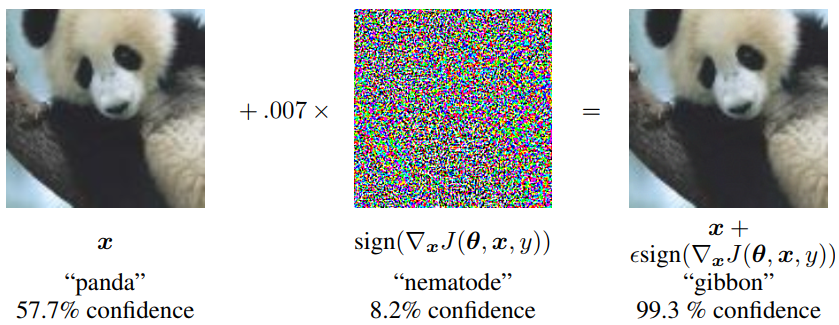
\includegraphics[width=0.7\textwidth]{adversarial.PNG}
  \caption{An example of AE: after adding a rubbish pattern to the original image, the model gives out another prediction with extremely high confidence. Credit: \cite{goodfellow2014explaining}}
  \label{fig:AE}
\end{figure}

By generating CFs, how do we avoid  ``gaming'' the system like the AEs? At first glance, it is impossible to distinguish them in practice because their mathematical principles are almost the same. Both required a different prediction result, and both need the perturbation to be small. But fortunately, there is one way out, which is the definition of ``near''. AEs need a perturbed input that is near to the original one because the perturbation should be not noticeable, while CFs need a near input so that the user is able to comprehend the main difference. In the case of CFs, the minimality of perturbation is not as important as for AEs, and it is enough to find inputs close enough to the original input that changes the classification in the desired way \cite{CFandAE}. The nearest CF explanations introduced in section \ref{sec:generation} are able to find CFs that are \emph{semantically} meaningful in distance function between different examples, but their benefits to the users are questionable.

Are nearest CF explanations wrong? Actually, ``counterfactual explanation'' is a broad topic, under which fall at least two groups of literature. Let's recap the two basic requirements of CFs here: a CF is a close input to the original input with a different prediction, i.e. equation \ref{eq:watcher}. Some authors develop their method under this assumption (e.g. \cite{certifai,watcher2017,DiCE}), and don't mention how to distinguish CFs generated by their purposed methods from AEs. Meanwhile, other authors expected more under this topic (e.g. \cite{prototype}), and they develop methods that prefer ``feasible'' solutions. Both groups, however, are a part of the big topic. Even though the latter sounds more favorable to a user, it is hard to exclude the former out of CF explanations. \citeauthor{CFandAE} \cite{CFandAE} has divided CF methods into two categories, namely \emph{contesting CF} and \emph{feasible CF}. The author argues that while the feasible CFs are useful in providing the user an actionable solution, the contesting CFs are useful in contesting a decision and therefore are similar to AEs. The author also clarifies the common misconceptions, pointing out that CFs are not equal to AEs, and feasible CFs are not all about CF explanation. In one word, $AE\approx contesting\ CF\subseteq CF$.
 \subsection{Lack of Actionability}
Consider the loan lending example again, an explanation may be ``You will be offered the loan if you decrease your age by three and change the education level to master.'' This explanation is certainly plausible (the bank system has seen someone who is younger but with a higher degree), but not actionable because the user could do nothing to improve his situation. A common criticism of nearest CF explanation methods is that they only answer the question of \emph{``what could have been done in the past''}, while the original aim of CF explanation should be \emph{``what should be done in the future''} \cite{algorithmicrecourse}.

There is a general agreement that causal constraints need to be taken into consideration for a feasible CF \cite{algorithmicrecourse}. Specifically, these constraints may include but are not limited to:
 \begin{itemize}
   \item Unary Causality Constraints: for example, age can not decrease with time.
   \item Binary Causality Constraints: other notations of this term are feature correlation \cite{preservingCausal} or downstream effects \cite{algorithmicrecourse}. For example changing the education level without an increase in age is not possible \cite{DiCE}.
   \item True Causality Connection: avoid spurious connections between a feature with the final prediction. For example, the higher salary one earns, the more dogs he can afford. But for loan approval the salary should be the only deciding feature, the model should not suggest a solution like ``if you raise one more dog, you will be offered with the loan'' \cite{diffThatMakesDiff}.
 \end{itemize}

What's more, it is worth mentioning that each CF is unique and user-specific. Besides the causal constraints, there may be also user-defined constraints, which the user is able to do but not willing to do, for example changing the city \cite{preservingCausal}. However, for the following discussion, these constraints are excluded to lay the main focus on causality.

%If these additional requirements are not fulfilled, the explanation can not be distinguished from an AE clearly and easily leaves an impression of deceiving the model. However, these additional requirements are rarely satisfied by the nearest CF methods. \cite{DiCE} has used a post-hoc filter to pick out the feasible explanations, but this is not the optimal solution. To generate feasible CFs, there is a general agreement that causal models, namely the effect of changing a variable on other variables, is a promising way out \cite{algorithmicrecourse}.

%%Nearest explanation answers the question ``what could have been done'', while casualty explanation answers ``what to do now'' 